


\textcolor{red}{The title says "Cold" but all the electronic, cold and warm, is described}


%%%%%%%%%%%%%%%%%%%%%%%%%%%%%%%%%%%%%%%%%%%%%%%%%%%%%%%%%%%%
\subsection*{Cryostat feed through}
%%%%%%%%%%%%%%%%%%%%%%%%%%%%%%%%%%%%%%%%%%%%%%%%%%%%%%%%%%%%
The feedthrough (FT) card developed for LArIAT is sandwiched between an ASA flange and cap, and sealed with o-rings. A stiff mechanical structure and backplane-style connectors support the FT card and allow for the WRD-48 cards to be plugged directly into it. Such an arrangement facilitates the assembly and potential repair work while reducing the amount of cables and connectors needed.

\begin{figure}[htbp]
 \centering
 \includegraphics[width=0.5\textwidth]{figures/FT_drawings.png}
\caption{
Drawing of LArIAT feed through and Warm Receiver Driver crate. 
} 
\label{pic:FeedthroughElectronics}
\end{figure}

The FT card is built as an 8-layer PCB with dimensions 254~mm $\times$ 432~mm. The outer layers of the card are mostly uninterrupted ground planes to increase noise immunity. The internal traces are built with relatively large 12~mil design rules to enhance manufacturing yield and physical robustness. Signal on adjacent layers are staggered to reduce capacitive cross-talk couplings, and ground fills are provided whenever possible on all copper layers.

Supporting the FT card is a mechanical structure that is rooted on the cryostat flange. The overall assembly of the card, the ten WRD-48 cards, and the WRD card cage is light enough to be safely cantilevered from the cryostat flange. The backplate of the structure is a solid copper sheet which is electrically connected with the cryostat flange though lock washers and also connected to the FT card through 40 conductive standoffs. The copper plate and the cryostat flange are defined as the electrical ground of the TPC readout electronics.

%%%%%%%%%%%%%%%%%%%%%%%%%%%%%%%%%%%%%%%%%%%%%%%%%%%%%%%%%%%%
\subsubsection*{CMB-48 card details}
%%%%%%%%%%%%%%%%%%%%%%%%%%%%%%%%%%%%%%%%%%%%%%%%%%%%%%%%%%%%
Each CMB-48 card holds 3 LArASICs. The card provides electrical connection to the LArIAT TPC wires and mechanical connection to the TPC structure. The CMB-48 board is located inside the cryostat and is thus inaccessible during data-taking periods. The board is designed to minimize the source of electrical noise, the risk of failure due to thermal stress, and the risk of component failure.

%%%%%%%%%%%%%%%%%%%%%%%%%%%%%%%%%%%%%%%%%%%%%%%%%%%%%%%%%%%%
\subsubsection*{WRD-48 card details}
%%%%%%%%%%%%%%%%%%%%%%%%%%%%%%%%%%%%%%%%%%%%%%%%%%%%%%%%%%%%
The WRD-48 cards are designed to be paired one-to-one with the CMB-48 cards inside the cryostat.The WRD-48 cards hold 48 channels of single-ended to differential analog amplifiers to transmit the TPC signals to the distant digitizers. These cards also provide low-noise power regulation, digital signal conditioning, front-panel diagnostic LEDs and voltage monitor ports, and an on-board test-pulse generator. 

%%%%%%%%%%%%%%%%%%%%%%%%%%%%%%%%%%%%%%%%%%%%%%%%%%%%%%%%%%%%
\subsection*{D2S-64 card details}
%%%%%%%%%%%%%%%%%%%%%%%%%%%%%%%%%%%%%%%%%%%%%%%%%%%%%%%%%%%%
The D2S-64 cards convert the differential analog signals from the WRD-48 cards to single-ended signals and drive these signals into the $50 \Omega$ input impedance of the CAEN V1740 digitizers.

The LArIAT data acquisition system is triggered to read out the digitizing buffers by a CAEN V1495 module. The V1495 is a powerful, easily configurable coincidence module featuring a user-programmable FPGA.  Sixteen logical inputs (upgraded to 32 in Run-III) are sampled on a 10~ns clock, checking for matches to any of the sixteen user-defined patterns in the trigger menu.  If a given trigger pattern is satisfied for two consecutive clock ticks, that pattern fires. 

NIM-standard logic pulse inputs to the trigger decision come from any of the instruments in the experiment, in principle; trigger inputs are derived from beam instruments, from the cosmic ray taggers, and from the cryostat's scintillation detectors. LArIAT takes full advantage of the trigger card's great flexibility.  As conditions change and innovations are gradually made to LArIAT's data-taking process, improvements are made to the trigger input designs and the combinations of inputs which define trigger patterns for the V1495.  The configuration of the trigger inputs is automatically logged in a database at the start of each run as part of the DAQ configuration, along with the rest of the XML configuration file for the V1495.

\subsubsection{Inputs to the Trigger System}

Two primary inputs to the trigger card are from the time of flight (see Sec.~\ref{sec:TOF}) and the wire chamber (see Sec.~\ref{sec:MWPC}) systems in the tertiary beamline.  Coincidence of activity in both of these systems strongly suggests that a charged particle has made the journey down the tertiary beam line from the copper target to the LArTPC in the cryostat, and that we will have a measure of its momentum and its velocity. PMT pulses from the time of flight system each pass through a 
%FIXME WHAT MODEL linear fanout?
linear fan-out, one output of which is threshold discriminated by a
%FIXME WHAT MODEL
discriminator to produce a NIM logic pulse for use in trigger logic.  On each of the upstream or downstream TOF paddles, we form a coincidence to within 20~ns of pulses from all the PMTs observing that same block of scintillator.  The upstream paddle coincidence signal is delayed 20~ns to allow any approximately lightspeed particles to travel 6.5~m to the downstream paddle.  The same upstream paddle coincidence signal is also widened to 100~ns to allow for slow-traveling (high-mass) particles.  Coincidences of these upstream and downstream TOF trigger input signals can be made in the V1495 trigger card.

Each wire chamber is read out by four multi-hit TDCs (time to digital converters), with sixty-four wires per TDC and two TDCs per plane (one horizontal and one vertical).  The TDCs each provide a logical ``fast'' OR of their inputs, indicating that one or more of their sixty-four wires went over the settable threshold.  Using NIM logic units, the OR of the horizontal wires and the OR of the vertical wires are input to a coincidence unit for each wire chamber, providing a single logical pulse for each of the four wire chambers, indicating that at least one horizontal wire and one vertical wire saw significant signal.  The single culminating logical pulses from each of the four wire chambers make up the first four inputs to the V1495 trigger card.  Within the user-programmable FPGA, the V1495 looks for the coincidence within 20~ns of at least three of these four specially-treated logical inputs.

Another primary input to the trigger card is from the cosmic towers (see Section~\ref{sec:CosmicRayPaddle}). To capture cosmic ray events in which a minimally ionizing cosmic ray muon crossed the TPC along the body diagonal, NIM modules form the logical coincidences from the two cosmic towers, one upper and one lower paddle assembly, in each combination.  The OR of these is provided as an input to the V1495. 

Three important logic pulses are derived from the timing of the beam.  These include a pulse in a brief window before the beam, a pulse indicating that the beam is on, and a pulse which defines the beam-free period which may be used for collecting cosmic-ray events.  An adjustable pulser is a fourth trigger input which does not depend on any particular activity in the experiment hall,  useful for collecting background events with zero bias. 

The PMTs observing liquid argon scintillation light (see Section \ref{sec:PhotonSystem}) produce pulses which form the foundation of several interesting trigger inputs.  Thresholding a copy of each PMT pulse (after amplification), and requiring a coincidence of pulses within $\sim$20~ns, creates simple trigger inputs indicating ionizing radiation was produced in the TPC.  This scintillation logic pulse is used to initiate a gate which spans the length of the TPC drift time, creating a logic signal which is remains ``on'' while significant drift charge may still be present in the TPC.  In addition, requiring a delayed coincidence of two subsequent scintillation logic pulses, separated by a variable length of time ranging from 300~ns to 7~$\mu$s, is used to create a trigger input to select events where a cosmic muon stops and decays to a Michel electron in the TPC.  A few different versions of this light-based trigger were implemented throughout the course of LArIAT's run time to allow reconstruction and calorimetric studies of Michel electrons. Figure~\ref{michel_logic} shows a schematic diagram of the logic comprising the Michel electron trigger. 

\begin{figure}
\includegraphics[width=\textwidth]{figures/trigger_michellogic.png}
\caption{\label{michel_logic}A schematic diagram of the trigger logic used to select Michel electron events during the cosmic readout window of the LArIAT supercycle.  The two PMT signals refer to the Hamamatsu (``HMM'') and ETL PMTs described in Section~\ref{sec:PhotonSystem}.  For some data-taking periods in Run-II, un-amplified pulses were discriminated at 180 mV to act as a veto on events that may saturate the dynamic range of the V1751 digitizer.  The discriminator thresholds used on the amplified (x10) PMT signal copies (\emph{ThA}, \emph{ThB}) as well as the Gate Delay period, were adjusted between run periods while experimenting with different configurations.}
\end{figure}

Further trigger inputs come from the beam line instrumentation behind the LArTPC cryostat, the PMTs of the Punch-Through scintillator paddles and those of the scintillator paddles instrumenting the Muon Range Stack.  The PMT pulses of all four of the broad-faced Punch Through paddles are discriminated to form logic pulses.  A single logic pulse is formed from these, indicating activity in at least two overlapping paddles at the rear of cryostat, before the steel block of the range stack.  PMT pulses from the Muon Range Stack are amplified and threshold discriminated.  These MuRS paddle pulses are then combined as in the Punch Through, creating single-bit indicators for each of the four instrumented layers that at least one pair of overlapping scintillator paddles sent signals within a 20~ns coincidence window.

\subsubsection{Trigger Decision and Issuance}

The V1495 may be configured to have up to sixteen trigger patterns and sixteen veto patterns, based on the trigger input signals.  A trigger pattern is defined as the AND of one or more defined inputs, and may include the NOT of the AND of further inputs.  Veto patterns are independently defined in the same way, but they have a very different effect.  When any of the trigger patterns fire, a ``fast trigger'' signal is issued and an adjustable countdown is initiated.  If the countdown completes without a veto pattern firing, the ``slow trigger'' signal is also issued and on a distinct hardware channel. Otherwise, if a veto pattern fires during the countdown, the slow trigger signal is vetoed.  

The fast trigger signal prompts readout of all the `short' data buffers, which include the V1751 modules, the V1495 itself, and the MWPC controller.  The V1751 buffers typically contain digitized PMT signals from the time of flight and cryogenic light collection detectors. Readout of the TPC wire signals, which are much longer and more numerous, is only prompted at the issuance of the slow trigger.


\subsection*{Signal Digitization}

Signals from all photodetectors are routed from the side-flange of the cryostat to NIM fan-outs to provide the 50-Ohm termination needed to minimize reflections along the cables. Copies of the PMT signals are made to aid in several light-based triggers, and copies of all signals are then recored into data using CAEN V1751 digitizer boards with 1~GHz sampling rate.

%------------------------------------------
\begin{figure}
\centering
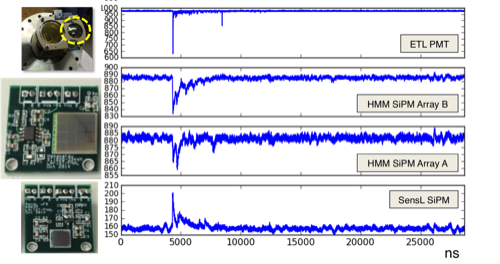
\includegraphics[width=0.8\textwidth]{figures/lightsys_signals.png}
\caption{Some example signals, in ADC units, from LArIAT photodetectors for a triggered cosmic Michel electron event.}
\label{lightsys_signals}
\end{figure}
\begin{figure}
\centering
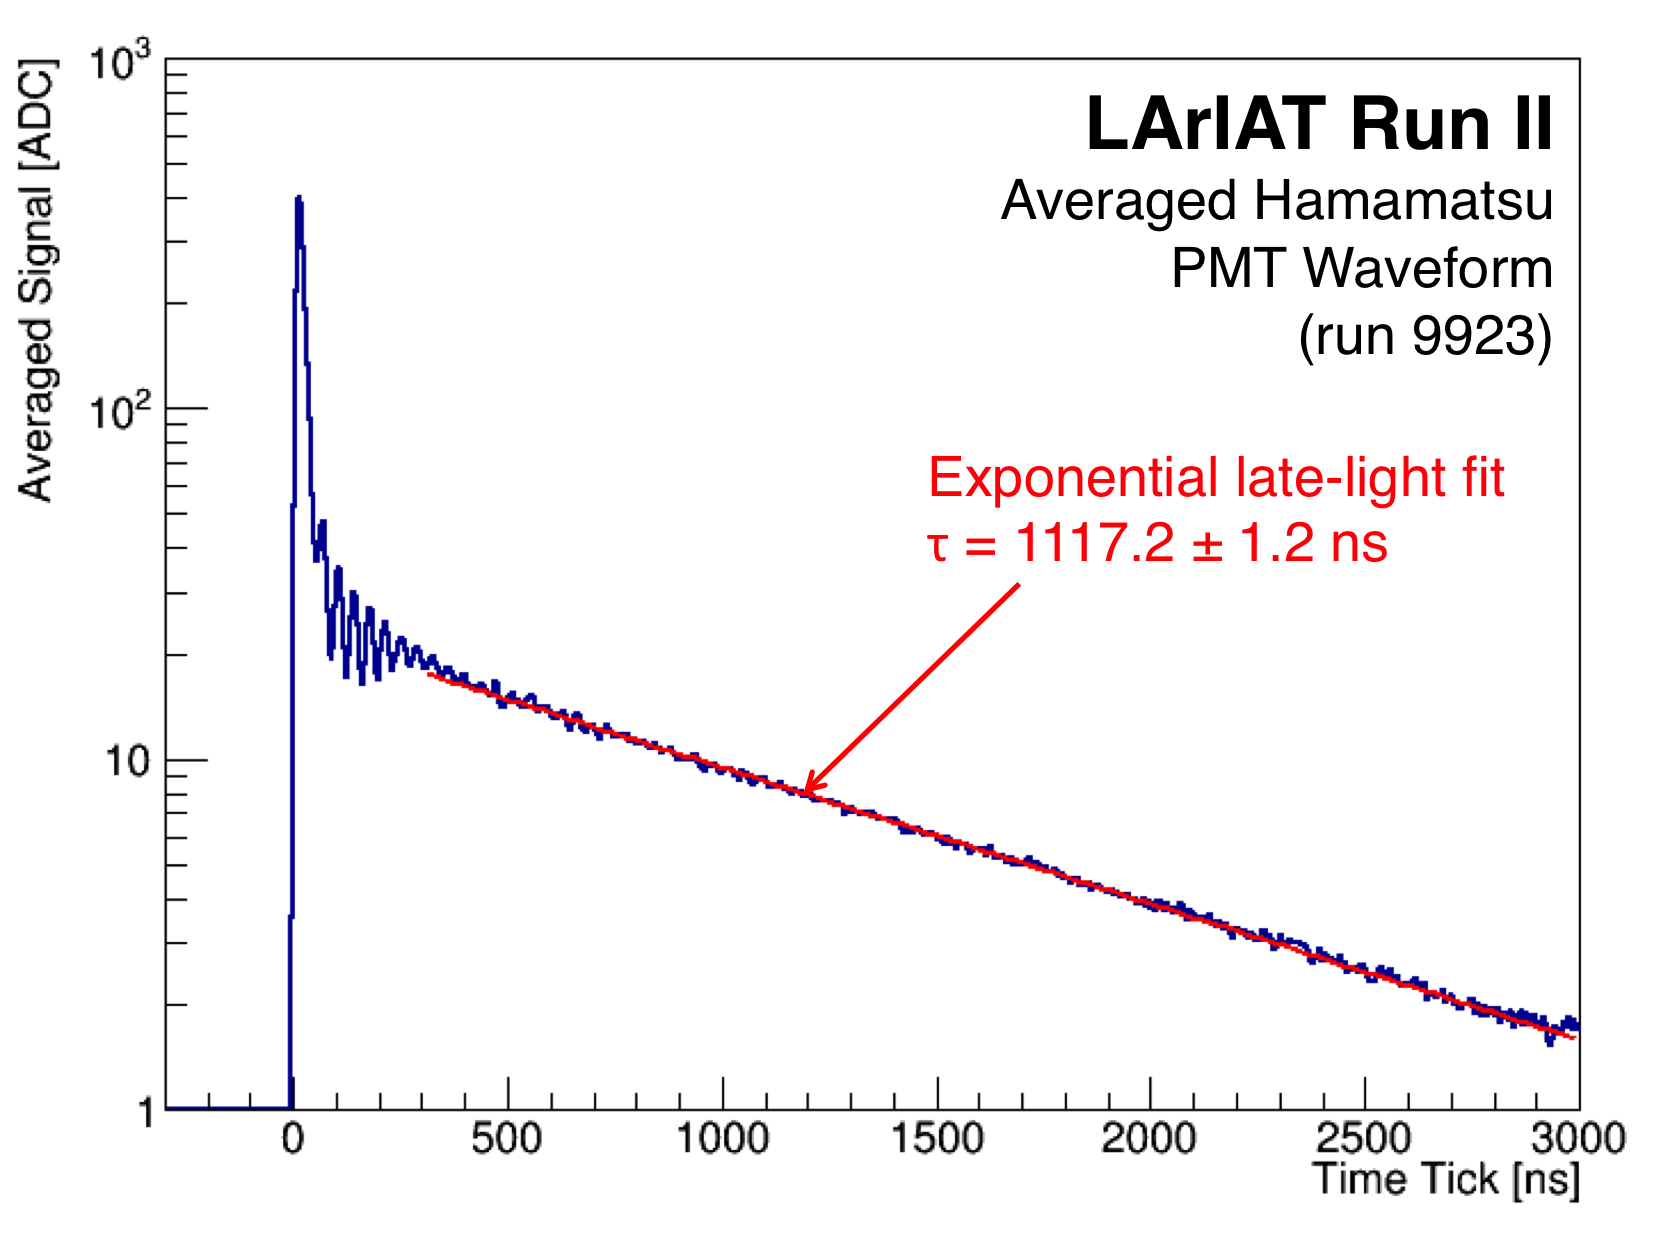
\includegraphics[width=0.6\textwidth]{figures/lightsys_avewfm_hmm.png}
\caption{\label{wfm_hmmpmt}An example of an averaged inverted waveform of the Hamamatsu PMT after event-by-event noise removal and overshoot correction.  Data was taken from a small subset of events from Run-II.  In this example, a falling exponential is fit to the signal region from 300~ns to 3~$\mu$s following the onset of the pulse to extract the late-light component lifetime $\tau$ = 1117~ns.}
\end{figure}
%------------------------------------------

\subsection*{Nitrogen Contamination Measurement Using Light}

The light detection system can also be used to derive information about the nitrogen (N2) contamination in liquid argon. The influence of N2 on liquid argon scintillation light emission has been observed in the WArP experiment~\cite{WARP-nitrogen}. With a higher N2 concentration, the observed decay time of the liquid argon slow component decreases significantly, from over 1~$\mu$s to hundreds of nanoseconds. In this measurement, waveforms recorded by the ETL PMT in Run-I, selected to cover periods of varying N2 concentrations (as measured by the external sensor in Figure~\ref{light_nitro}), were analyzed. An exponential fit was performed to estimate the decay time of the slow light component. Results, shown in Figure~\ref{light_nitro}, were compared with the model from the WArP paper~\cite{WARP-nitrogen}.

%------------------------------------------
\begin{figure}
\includegraphics[height=0.2\textheight]{figures/nitrosensor.jpeg}
\hspace{0.5cm}
\includegraphics[height=0.2\textheight]{figures/nitro_qt.jpeg}
\label{light_nitro}
\caption{Concentration of N2 in LArIAT as measured by an external sensor in Run-I (left), and results of fitting exponential models to waveforms recorded by the ETL PMT compared with the model from WArP~\cite{WARP-nitrogen} (red line).}
\end{figure}
%------------------------------------------
